%File: formatting-instruction.tex
\documentclass[letterpaper]{article}
\usepackage{aaai}
\usepackage{times}
\usepackage{helvet}
\usepackage{courier}
\usepackage{algpseudocode}
\usepackage[ruled]{algorithm}
\usepackage{url}
\usepackage{framed}
\usepackage{amsfonts,amsmath,amsthm,amssymb}
\usepackage{graphicx}
\usepackage{url}
\usepackage{color}

\newtheorem{lemma}{Lemma}
\frenchspacing
\pdfinfo{
/Title (MCTS Based on Simple Regret)
/Subject (AAAI Publications)
/Author (AAAI Press)}

\setcounter{secnumdepth}{0}  
\newcommand {\mean} {\ensuremath {\mathop{\mathrm{mean}}}}
\newcommand {\median} {\ensuremath {\mathop{\mathrm{median}}}}
\newcommand {\N} {\ensuremath {\mathcal{N}}}
\newcommand {\IE} {\ensuremath {\mathbb{E}}}
\newcommand {\cov} {\ensuremath {\mathop{\mathrm{cov}}}}
\newcommand {\BEL} {\ensuremath {\mathop{\mathrm{BEL}}}}

\newtheorem{dfn}{Definition}
\newtheorem{thm}{Theorem}
\newtheorem{lmm}{Lemma}
\newtheorem{crl}{Corollary}

\title{MCTS Based on Simple Regret}
\author {David Tolpin, Solomon Eyal Shimony \\
Department of Computer Science, \\
Ben-Gurion University of the Negev, Beer Sheva, Israel \\
\{tolpin,shimony\}@cs.bgu.ac.il}
\begin{document}

\maketitle

\begin{abstract}
UCT, a state-of-the art algorithm for Monte Carlo tree search (MCTS)
in games and Markov decision processes, is based on UCB, a sampling
policy for the Multi-armed Bandit problem (MAB) that asymptotically
minimizes the cumulative regret.  However, search differs from MAB in
that in MCTS it is usually only the final ``arm pull'' (the actual
move selection) that collects a reward, rather than all ``arm pulls''.
Therefore, it makes more sense to minimize the simple regret, as
opposed to the cumulative regret. We begin by introducing policies for
multi-armed bandits with lower finite-time and asymptotic simple
regret than UCB, using it to develop an algorithm (USRT) for MCTS
which outperforms UCT empirically.

We then observe that optimizing the sampling process is itself a
meta-reasoning problem, a solution of which can use value of
information (VOI) techniques.  Although the theory of VOI for search
exists, applying it to MCTS is non-trivial, as typical myopic
assumptions fail. Lacking a working VOI theory for MCTS, we
nevertheless propose a sampling scheme that is ``aware'' of VOI,
achieving an algorithm that in empirical evaluation outperforms USRT,
as well as UCT.
\end{abstract}

\section{Introduction}

Monte-Carlo tree sampling, and especially a version based on the
UCT formula \cite{Kocsis.uct} appears in numerous search applications,
such as \cite{Eyerich.ctp}. Although these methods are shown to be successful empirically,
most authors appear to be using the UCT formula ``because it has been shown
to be successful in the past'', and ``because it does a good job of
trading off exploration and exploitation''. While the latter statement may be
correct for the multi-armed bandit and for the UCB method \cite{Auer.ucb},
we argue that it is inappropriate for search. The problem is not that
UCT does not work; rather, we argue that a simple reconsideration from basic
principles can result in schemes that outperform UCT.

The core issue is that in search (especially for adversarial search
and for ``games against nature'' - optimizing behavior under
uncertainty) the goal is typically to either find a good (or optimal)
strategy, or even to find the best first action of such a policy. Once
such an action is discovered, it is not beneficial to further sample
that action, ``exploitation'' is thus meaningless for search
problems. Finding a good first action is closer to the pure
exploration variant, as seen in the selection problem
\cite{Bubeck.pure,TolpinShimony.blinkered}. In the selection problem,
it is much better to minimize the \emph{simple} regret.  However, the
simple and the cumulative regret cannot be minimized simultaneously;
moreover, \cite{Bubeck.pure} shows that in many cases the smaller the
cumulative regret, the greater the simple regret.

We begin with introduction of several sampling schemes with better
bounds for the simple regret on sets. We then extend the resutls to
sampling in trees by combining the proposed sampling schemes on the
first step of a rollout with UCT during the rest of the
rollout. Finally, we empirically evaluate the performance of the
proposed sampling schemes on sets of Bernoulli arms, in randomly
generated trees, and on the sailing domain.

\section{Related Work}
\label{sec:related-work}

Efficient algorithms for Multi-Armed Bandits based on
distribution-independent bounds, in particular UCB1, are introduced in
\cite{Auer.ucb}. The UCT algorithm, an extension of UCB1 to
Monte-Carlo Tree Search is described in \cite{Kocsis.uct}. Pure
exploration in Multi-armed bandits is explored in
\cite{Bubeck.pure}. On the one hand, the paper proves certain upper
and lower bounds for UCB1 and uniform sampling, showing that an upper
bound on the simple regret is exponential in the number of samples for
uniform sampling, while only polynomial for UCB1. On the other hand,
empirical performance of UCB1 appears to be better than of uniform
sampling. 

The principles of bounded rationality appear in
\cite{Horvitz.reasoningabout}. \cite{Russell.right} provided a formal
description of rational metareasoning and case studies of applications
in several problem domains. One obstacle to straightforward
application of the principles of rational metareasoning to Monte-Carlo
sampling is the metagreedy assumption, according to which samples must
be selected as though at most one sample can be taken before an action
is chosen. In Monte-Carlo sampling, the value of information of any
single sample in a given search state is often zero, so a different
approximating assumption must be used instead.

\section{Sampling Based on Simple Regret}
\label{sec:results}

In the Multi-armed Bandit problem \cite{Vermorel.bandits} we have a set
of $K$ arms. Each arm can be pulled multiple times. When the $i$th arm
is pulled, a random reward $X_i$ from an unknown stationary
distribution is returned.  The reward is bounded between 0 and 1.

\begin{dfn}
The \textbf{simple regret} of a sampling policy for the Multi-armed Bandit
Problem is the expected difference between the best expected reward
$\mu_*$ and the expected reward $\mu_j$ of the empirically best arm
$\overline X_j=\max_i\overline X_i$:
\begin{equation}
\label{eq:simple-regret}
\IE r=\sum_{j=1}^K\Delta_j\Pr(\overline X_j=\max_i\overline X_i)
\end{equation}
where $\Delta_j=\mu_*-\mu_j$.
\end{dfn}

Strategies that minimize the simple regret are called pure exploration
strategies \cite{Bubeck.pure}. Such strategies are used to select the
best arm, and, by extension, the best action in MCTS. MCTS is used to
solve Markov Decision Processes (MDP) approximately. An MDP is defined
by the set of states $S$, the set of actions $A$, the transition table
$T(s, a, s')$, the reward table $R(s, a, s')$, the initial state $s$
and the goal state $t$: $(S, A, T, R, s, t)$ \cite{Russell.aima}.
MCTS explores an MDP by \emph{rollouts}---trajectories from the
current state to a state in which a termination condition is satisfied
(either the goal state, or a cutoff state for which the reward is
evaluated approximately). The UCB algorithm (that attempts to minimize
the cumulative regret) \cite{Auer.ucb} had been extended into the tree
search sampling scheme known as UCT \cite{Kocsis.uct}.

UCT performance can be improved by combining UCB with a sampling
scheme that minimizes the simple regret of selecting an action at the
current root node. Indeed, the algorithm must select an action with
the minimum regret \emph{given the assumption that after performing the selected action
the algorithm performs optimally}, which corresponds to maximizing the
value of partial information \cite{Russell.aima}. Therefore, an
improved allocation scheme would
\begin{itemize}
\item maximize the value of partial
information by sampling actions to
minimize the \textbf{simple} regret
of the selection at the current root node, and
\item as the goal of sampling in deeper tree nodes is estimating the value of
a node, rather than selection, it makes sense to
minimize the \textbf{cumulative} regret of the rollouts from the second
step onwards. 
\end{itemize}
Ultimately, an ``optimal'' sampling in the meta-reasoning sense should
be used at the first step in the above scheme. Nevertheless, this task
is daunting for the following reasons:
\begin{itemize}
\item Defining the cost of a sample is not easy, and even if we simply
  use time-cost as an approximation, we get an intractable
  meta-reasoning problem.
\item Applying the standard myopic and subtree independence
  assumptions, we run into serious problems. Even in the standard
  selection problem \cite{TolpinShimony.blinkered}, we get a
  non-concave utility function and premature stopping of the
  algorithm. This is due to the fact that the value of information of
  a single measurement (analogous to a sample in MCTS) is frequently
  less than its time-cost, even though this is not true for multiple
  measurements.  When applying the selection problem to MCTS, the
  situation is exacerbated.  The utility of an action is usually
  bounded, and thus in many cases a single sample may be insufficient
  to change the current best action, \emph{regardless} of its
  outcome. As a result, we frequently get a \emph{zero} ``myopic''
  value of information for a single sample.
\end{itemize}
As the ultimate goal is extremely difficult
to achieve, and even harder to analyze, we introduce
simple schemes more amenable to analysis, and compare
them to UCB (on sets) and UCT (in trees). 

\subsection{Sampling on Sets}
\label{sec:sampling-on-sets}

\begin{dfn} Scheme $\mathbf{UCB(\alpha)}$ repeatedly pulls arm $i$ that maximizes 
upper confidence bound $b_i$ on the reward:
\begin{equation}
b_i=\overline X_i+\sqrt {\frac {\alpha \ln n} {n_i}}
\end{equation}
where $\overline X_i$ is the average reward obtained from arm $i$,
$n_i$ is the number of times arm $i$ was pulled, and $n$ is the total
number of pulls so far. \end{dfn} The best known upper bound on the simple
regret of UCB($\alpha$) is polynomially decreasing in the number of samples
(see \cite{Bubeck.pure}, Theorems~2,3).

An upper bound on the simple regret of uniform sampling is
exponentially decreasing in the number of samples (see
\cite{Bubeck.pure}, Proposition~1). However, empirically
UCB($\alpha$) yields a lower simple regret than uniform
sampling. 

We introduce here two sampling schemes with exponentially
decreasing upper bounds on the simple regret. The bounds
suggest that these schemes achieve a lower simple regret
than uniform sampling; indeed, this is confirmed
by experiments. 

We first consider $\varepsilon$-greedy sampling as a straightforward
generalization of uniform sampling:
\begin{dfn} The \textbf{$\mathbf{\varepsilon}$-greedy} sampling scheme
pulls the empirically best arm with probability $\varepsilon$ and any other
arm with probability $\frac {1-\varepsilon} {K-1}$. 
\end{dfn}

\begin{thm} Simple regret of the  $\varepsilon$-greedy
sampling scheme is asymptotically bounded from above as
\begin{equation}
\IE r_{\varepsilon\mbox{-}greedy}\le...
\end{equation}
the bound is minimized for $\varepsilon=\frac 1 2$.
\end{thm}

\begin{proof}[Proof sketch:] TODO
\end{proof}

\begin{dfn} Scheme $\mathbf{UCB_{\sqrt{\cdot}}(\alpha)}$ repeatedly pulls arm $i$ that
maximizes $b_i$:
\begin{equation}
b_i=\overline X_i+\sqrt {\frac {\alpha \sqrt n} {n_i}}
\end{equation}
where, as before, $\overline X_i$ is the average reward obtained from arm $i$,
$n_i$ is the number of times arm $i$ was pulled, and $n$ is the total
number of pulls so far. \end{dfn}

\begin{thm} Simple regret of the UCB$_{\sqrt{}}$($\alpha$) sampling
  scheme is asymptotically bounded from above as.
\begin{equation}
\IE r_{ucb\sqrt{\cdot}} \le ...
\end{equation}
\end{thm}
\begin{proof}[Proof sketch:] TODO
\end{proof}

\subsection{Sampling in Trees}
\label{sec:sampling-in-trees}

UCT \cite{Kocsis.uct} is a generalization of UCB for MCTS.  UCT
applies UCB at each step of a rollout.  We suggest an improvement on
UCT, which combines different sampling schemes on the first step and
during the rest of a rollout:
\begin{dfn}
The \textbf{SR+CR MCTS sampling scheme} selects an action at the
current root node according to a scheme suitable for minimizing 
simple regret (\textbf{SR}), such as $\frac 1 2$-greedy or UCB$_{\sqrt{\cdot}}$, and
then selects actions according to UCB, minimizing cumulative regret (\textbf{CR}).
\end{dfn}

Such two-stage sampling scheme outperforms UCT, and, additionally, is
significantly less sensitive to the tuning of the exploration factor
$\alpha$ of UCT, since the conflict between the need for a larger
value of $\alpha$ on the first step (simple regret) and a smaller
value for the rest of the rollout (cumulative regret)
\cite{Bubeck.pure} is resolved. In fact, a sampling scheme that uses
UCB at all steps but a larger value of $\alpha$ for the first step
than for the rest of the steps, outperforms UCT. The pseudocode of the
two-stage rollout is in Algorithm~\ref{alg:two-stage-mcts}.

\begin{algorithm}[t]
\caption{Two-stage Monte-Carlo tree search sampling}
\label{alg:two-stage-mcts}
\begin{algorithmic}[1]
\Procedure{Rollout}{node, depth=1}
  \If {\Call{IsLeaf}{node, depth}}
    \State \textbf{return} 0
  \Else
    \If {depth=1}
      \State action $\gets$ \Call{FirstAction}{node}
    \Else
      \State action $\gets$ \Call{NextAction}{node}
    \EndIf
    \State next-node $\gets$ \Call{NextState}{node, action}
    \State reward $\gets$ \Call{Reward}{node, action, next-node}
     \State \hspace{4em} + \Call{Rollout}{next-node, depth+1}
    \State \Call{UpdateStats}{node, action, reward}
  \EndIf
\EndProcedure
\end{algorithmic}
\end{algorithm}

\subsection{VOI-aware Sampling}

A further improvement can be achieved by computing or estimating the
value of information (VOI) of the rollouts and choosing a rollout that
maximizes the VOI. VOI of a rollout can be computed when the sample
distribution of an action is known up to the parameters, such as the
normal distribution with an unknown mean and/or
variance. Alternatively, the value of information can be estimated
from the set of samples, and the need to assume a particular shape of
the distribution can be lifted. In one realization of the latter
approach the VOI of performing an action is estimated as an
\emph{upper bound on the value of perfect information about an arm,
divided by the number of pulls of the arm}.
\begin{eqnarray}
VOI_\alpha&\approx&\frac {\overline X_\beta} {n_\alpha+1}
\exp\left(-2(\overline X_\alpha - \overline X_\beta)^2 n_\alpha\right)\\
VOI_i&\approx&\frac {1-\overline X_\alpha} {n_i+1}
\exp\left(-2(\overline X_\alpha - \overline X_i)^2 n_i\right),\; i\ne\alpha\nonumber\\
\mbox{where }\alpha&=&\arg\max_i \overline X_i\nonumber\\
             \beta&=&\arg\max_{i,\,i\ne\alpha} \overline X_i\nonumber
\end{eqnarray}
Early experiments with this approach demonstrated
significantly lower simple regret on a wide range of problems.

\section{Empirical Evaluation}
\label{sec:emp}

The results were empirically verified on Multi-armed Bandit instances,
on search trees, and on the sailing domain, as defined in
\cite{Kocsis.uct}. In most cases, the experiments showed lower average
simple regret for $\frac 1 2$-greedy an UCB$_{\sqrt{\cdot}}$ than for
UCB on sets, and for the SR+CR scheme than for UCT in trees.

\subsection{Simple regret in multi-armed bandits}
\label{sec:emp-mab}

Figure~\ref{fig:mab-simple-regret} presents a comparison of MCTS sampling
schemes on Multi-armed bandits. Figure~\ref{fig:mab-simple-regret}.a shows the search tree
corresponding to a problem instance. Each arm returns a random reward
drawn from a Bernoulli distribution. The search selects an arm
and compares the expected reward, unknown to the algorithm during the
sampling, to the expected reward of the best arm. For such problem
instances, the MCTS sampling schemes coincide with the selection
algorithms employed at the first step of a rollout.

Figure~\ref{fig:mab-simple-regret}.b shows the regret
vs. the number of samples, averaged over $10^4$ experiments for
randomly generated instances of 32 arms. 

For smaller numbers of samples, GCT achieves the best
performance; for larger numbers of samples, QCT outperforms GCT. QCT is
better than UCT everywhere except for very small numbers of samples. A
combination of GCT and QCT dominates UCT over the whole range.

\begin{figure}[h!]
  \begin{minipage}[c]{1.0\linewidth}
    \centering
    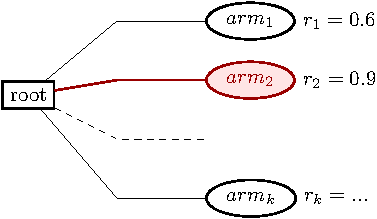
\includegraphics[scale=1.0]{onelevel-tree.pdf}\\
    a. search tree
    \vspace{1em}
  \end{minipage}
  \begin{minipage}[c]{1.0\linewidth}
    \centering
    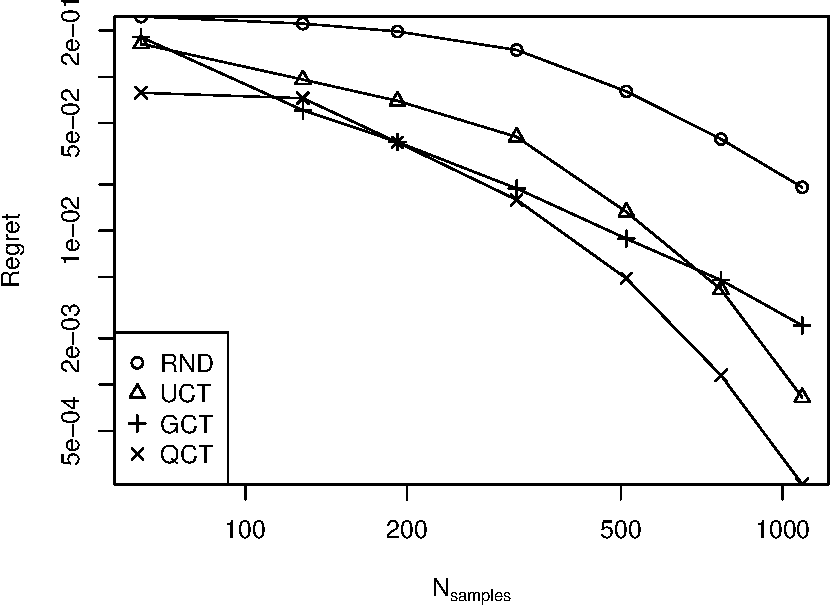
\includegraphics[scale=0.5]{flat-trilevel-k=64-uqb=8.pdf}\\
    b. regret vs. number of samples
  \end{minipage}
  \caption{Simple regret in MAB}
  \label{fig:mab-simple-regret}
\end{figure}

\subsection{Monte Carlo tree search}
\label{sec:emp-mcts}

The second set of experiments was performed on randomly generated
trees crafted in such a way that uniform random sampling selects a
direction at the root randomly. The degree of the root is a parameter of
the tree generator. The degree of all nodes at distance 1 from the
root is 2, and all nodes at distance 2 from the roots are leaves. The
average reward of two children of each node at distance 1 is
0.5. Thus, a uniform sampling scheme results in the same average reward for
all edges at the root, and an adaptive sampling scheme, such as UCT,
has to be used.

Figure~\ref{fig:mcts-regret} shows a sketch of the search tree
(Figure~\ref{fig:mcts-regret}.a) and the dependency of the regret vs. the
number of samples for trees with root degree 16
(Figure~\ref{fig:mcts-regret}.b) and 64 (Figure~\ref{fig:mcts-regret}.c). The
dependencies look differently from Multi-armed bandit instances, but
the algorithms exhibit a similar relative performance: either GCT or QCT
is always better than UCT, QCT dominates UCT everywhere
except for small numbers of instances. The advantage of QCT grows with
the number of arms.

\begin{figure}[h!]
  \begin{minipage}[c]{1.0\linewidth}
    \centering
    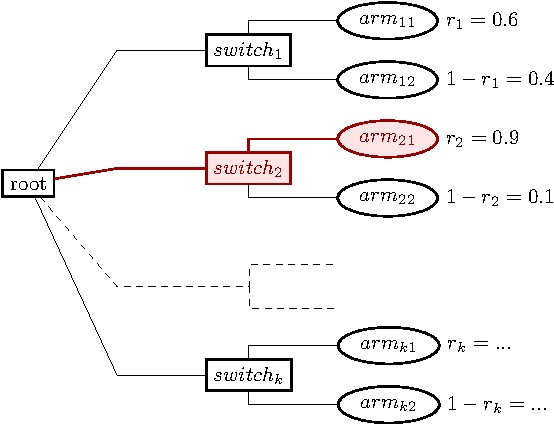
\includegraphics[scale=0.8]{twolevel-tree.pdf}\\
    a. search tree
    \vspace{1em}
  \end{minipage}
  \begin{minipage}[c]{1.0\linewidth}
    \centering
    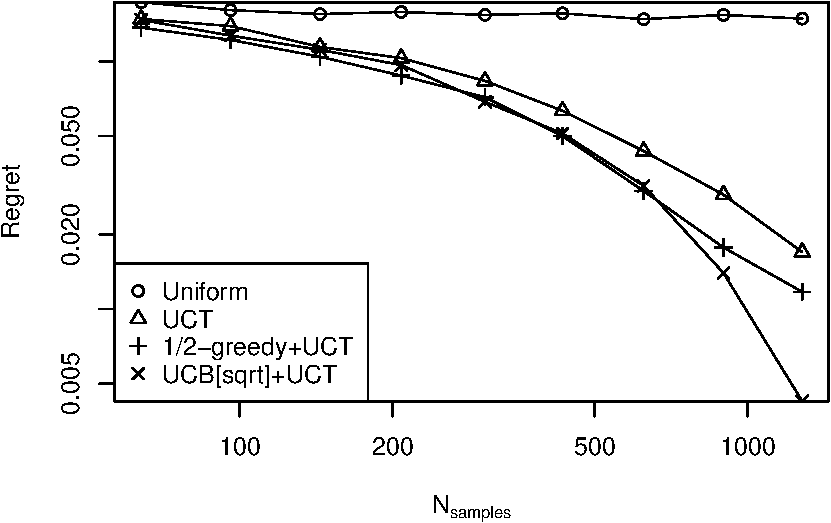
\includegraphics[scale=0.5]{tree-identity-k=16-uqb=8.pdf}\\ 
    b. 16 arms
    \vspace{1em}
  \end{minipage}
  \begin{minipage}[c]{1.0\linewidth}
    \centering
    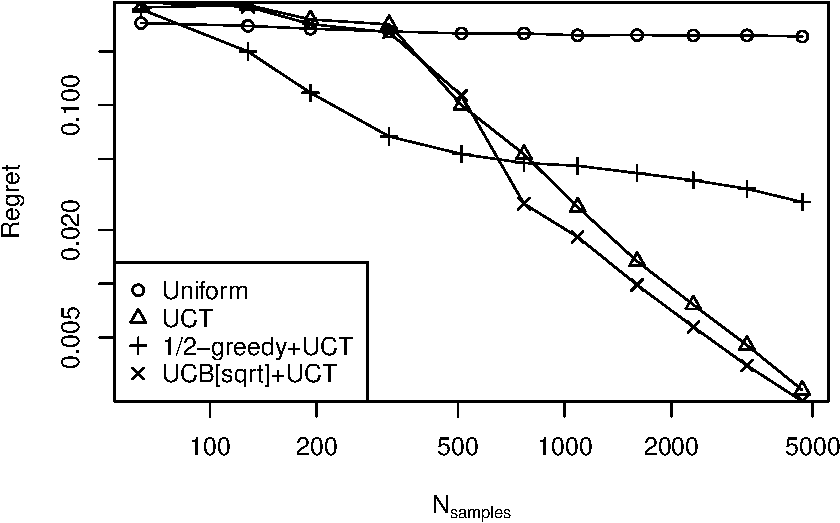
\includegraphics[scale=0.5]{tree-identity-k=64-uqb=8.pdf} \\
    c. 64 arms
  \end{minipage}
  \label{fig:mcts-regret}
  \caption{MCTS: a path to the best arm}
\end{figure}

\subsection{The sailing domain}
\label{sec:emp-sailing}

Figures~\ref{fig:sailing-cost-vs-nsamples}--\ref{fig:sailing-rcq-vs-factor}
show results of experiments on the sailing
domain. Figure~\ref{fig:sailing-cost-vs-nsamples} shows the regret
vs. the number of samples, computed for a range of values of
$\alpha$. Figure~\ref{fig:sailing-cost-vs-nsamples}.a shows the median
cost, and Figure~\ref{fig:sailing-cost-vs-nsamples}.b --- the minimum
costs. UCT is always worse than either $\frac 1 2$-greedy (GCT) or
QCT, and is sensitive to the value of $\alpha$: the median cost is
much higher than the minimum cost for UCT. For both $\frac 1 2$-greedy
and QCT, the difference is significantly less prominent.

\begin{figure}[h!]
  \begin{minipage}[b]{1.0\linewidth}
    \centering
    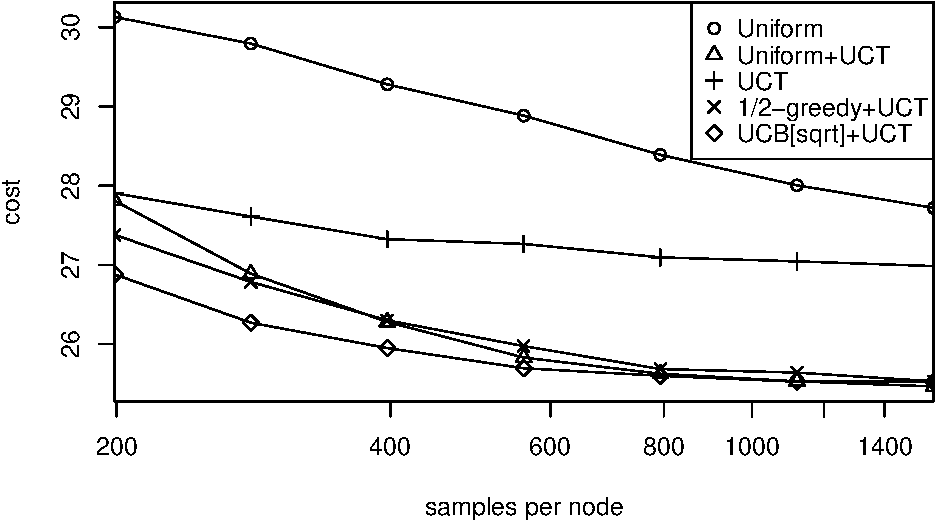
\includegraphics[scale=0.45]{costs-size=6-group=median.pdf}\\
    a. median cost
    \vspace{1em}
  \end{minipage}
  \begin{minipage}[b]{1.0\linewidth}
    \centering
    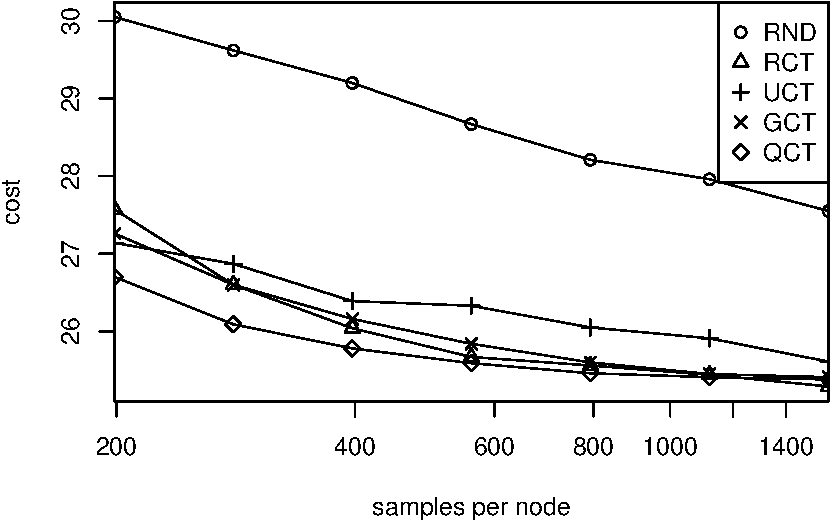
\includegraphics[scale=0.45]{costs-size=6-group=minimum.pdf}\\
    b. minimum cost
  \end{minipage}
  \caption{The sailing domain, $6\times 6$ lake, cost vs. number of rollouts}
  \label{fig:sailing-cost-vs-nsamples}
\end{figure}

Figure~\ref{fig:sailing-cost-vs-factor} shows the regret vs. the
exploration factor for different numbers of samples. QCT is always better than
UCT, and $\frac 1 2$-greedy is better than UCT expect for a small range of
values of the exploration factor $\alpha$. 

\begin{figure}[h!]
  \centering
  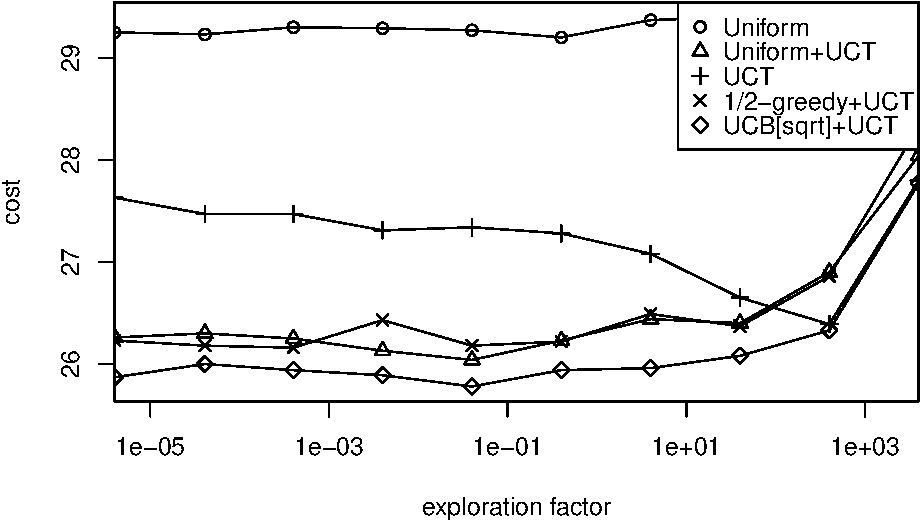
\includegraphics[scale=0.45]{costs-size=6-nsamples=397.pdf}\\
  a. 397 rollouts\\
  \vspace{1em}
  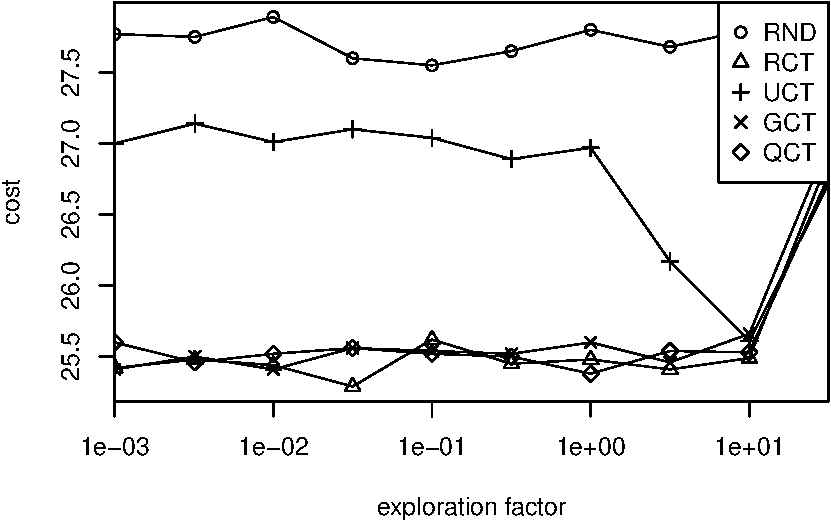
\includegraphics[scale=0.45]{costs-size=6-nsamples=1585.pdf}\\
  c. 1585 rollouts
  \caption{The sailing domain, $6\times 6$ lake, cost vs. factor}
  \label{fig:sailing-cost-vs-factor}
\end{figure}

Figure~\ref{fig:sailing-lake-size} shows the cost vs. the exploration
factor for lakes of different sizes. The relative difference between
the sampling schemes becomes more prominent when the lake size
increases.
\begin{figure}[h!]
   \centering
   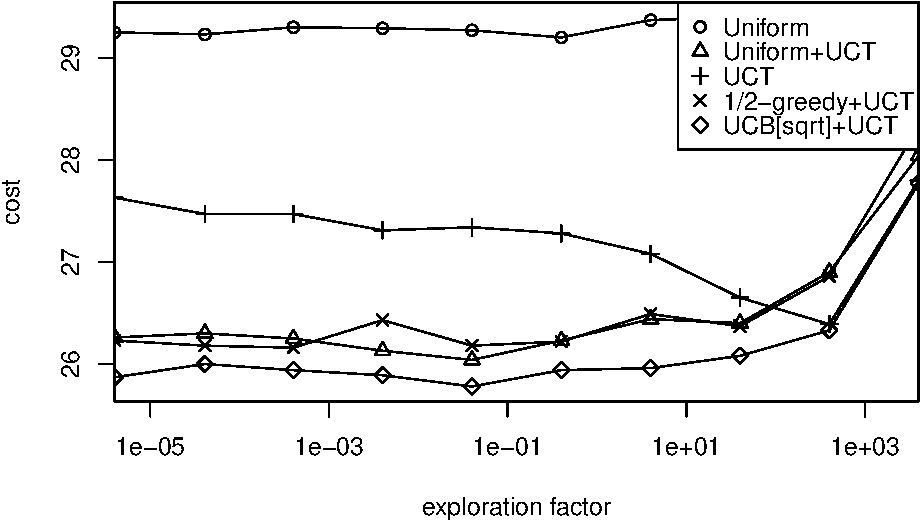
\includegraphics[scale=0.45]{costs-size=6-nsamples=397.pdf}\\
   b. $6\times 6$ lake \\
   \vspace{1em}
   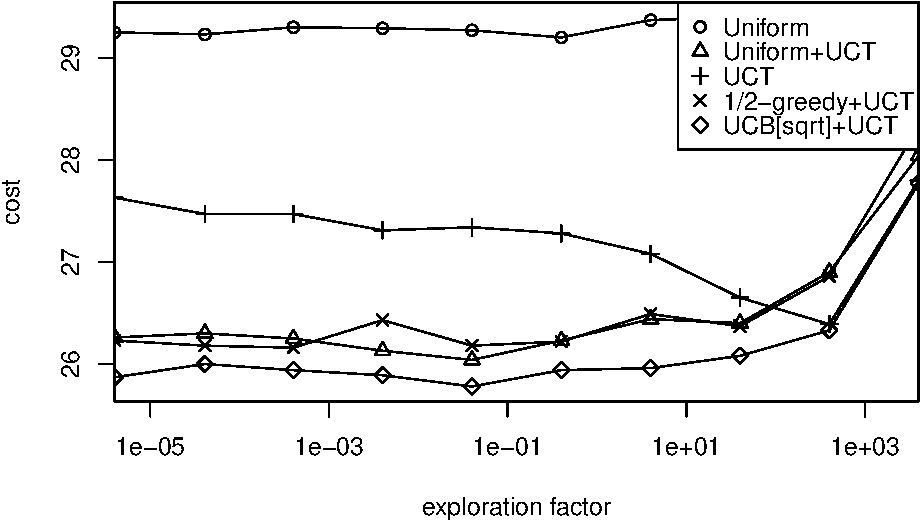
\includegraphics[scale=0.45]{costs-size=10-nsamples=397.pdf}\\
   c. $10\times 10$ lake
  \caption{The sailing domain, 397 samples, cost vs. factor}
  \label{fig:sailing-lake-size}
\end{figure}

Figure~\ref{fig:sailing-rcq-vs-factor} compares QCT with UCT with a
different exploration factor at the root (CCT). $\alpha$ for the rest of
the steps was chosen to ensure the best performance from earlier
experiments on the domain. Both algorithms exhibit similar dependency,
but as the number of samples grows, QCT achieves smaller average
regrets and is less sensitive to the choice of the value for $\alpha$ at
the first step.
\begin{figure}[h!]
  \centering
  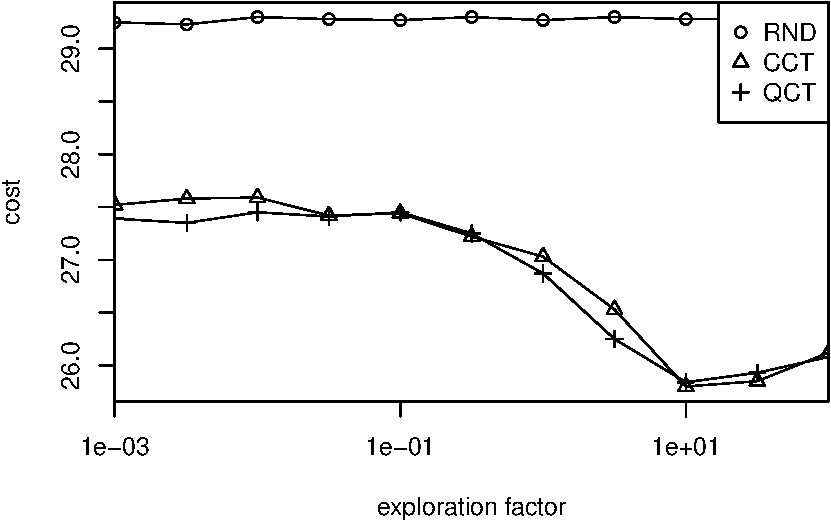
\includegraphics[scale=0.45]{rcq-size=6-nsamples=397.pdf}\\
  b. 397 rollouts\\
  \vspace{1em}
  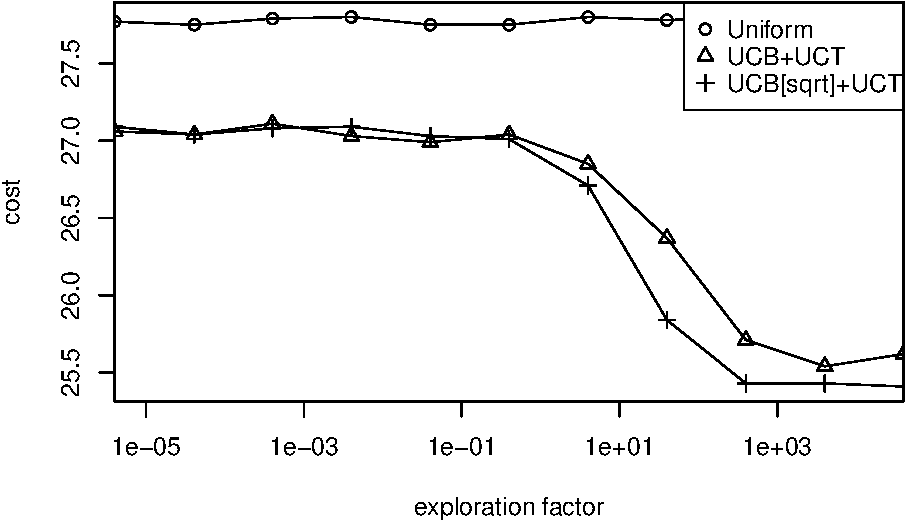
\includegraphics[scale=0.45]{rcq-size=6-nsamples=1585.pdf}\\
  d. 1585 rollouts\\
  \caption{The sailing domain, log vs. sqrt, $6\times 6$ lake}
  \label{fig:sailing-rcq-vs-factor}
\end{figure}

\section{Summary and Future Work}
\label{sec:summary}

The MTCS SR+CR scheme presented in the paper differs
from UCT at the first step of the rollout, when the `simple' selection
regret is minimized instead of the cumulative regret. Both the
theoretical analysis and the empirical evaluation provide evidence for
better general performance of the proposed scheme.

\section*{Acknowledgments}

The research is partially supported by Israel
Science Foundation grant 305/09, by the Lynne and William Frankel
Center for Computer Sciences, and by the Paul Ivanier Center for
Robotics Research and Production Management.

 \bibliographystyle{aaai}
\bibliography{refs}


\end{document}
